\documentclass{beamer}

\usetheme{Berlin}
\usecolortheme{Orchid}
\useoutertheme{miniframes}
\setbeamertemplate{navigation symbols}{}

\usepackage[utf8]{inputenc}
\usepackage[T1]{fontenc}
\usepackage{amsmath}
\usepackage{amssymb}
\usepackage{booktabs}
\usepackage{graphicx}
\graphicspath{{../images/}}

\usepackage{xcolor}
\usepackage{listings}
\usepackage{hyperref}
\usepackage{tikz}
\usetikzlibrary{arrows.meta,positioning,shapes.geometric,calc}

\lstset{
  language=Java,
  basicstyle=\ttfamily\small,
  keywordstyle=\color{blue},
  commentstyle=\color{gray},
  stringstyle=\color{teal},
  showstringspaces=false,
  columns=fullflexible,
  breaklines=true
}

% Per-slide source line (references shown on the slide itself).
\newcommand{\slidesources}[1]{%
  \vfill
  {\tiny\color{gray}\raggedright\sloppy\parbox{\linewidth}{Sources: #1}\par}%
}

% Unit-wise source strings for this subject (used by slides/notes).
% Path is relative to the lecture `latex/` folder (the compilation CWD).
% OOPS with Java (CSEG1044) — unit-wise sources
%
% These are short, student-facing reference strings intended to be used with:
%   - \slidesources{...}  (in beamer slides)
%   - \notesources{...}   (in lecture notes)
%
% Style inspiration: other subjects in My-Subjects/ use semicolon-separated sources
% and include an "accessed" date for web documentation.

\newcommand{\OOPSUnitISources}{Schildt, \textit{Java: A Beginner's Guide} (10e), McGraw-Hill (Java fundamentals + OOP basics).; Oracle Java Tutorials: Getting Started + Language Basics + Classes and Objects (accessed \today).; Java SE API docs (e.g., \texttt{String}, \texttt{Scanner}) (accessed \today).}

\newcommand{\OOPSUnitIISources}{Schildt, \textit{Java: The Complete Reference} (12e), McGraw-Hill (classes, inheritance, packages, interfaces).; Bloch, \textit{Effective Java} (3e), Addison-Wesley, 2018 (design choices; interfaces vs abstract classes).; Oracle Java Tutorials: Classes and Objects + Interfaces + Packages (accessed \today).; Java SE API docs (e.g., \texttt{Comparable}, \texttt{Runnable}) (accessed \today).}

\newcommand{\OOPSUnitIIISources}{Schildt, \textit{Java: The Complete Reference} (12e) (nested/inner classes, exceptions, threads, I/O).; Oracle Java Tutorials: Nested Classes + Exceptions + Concurrency + Basic I/O (accessed \today).; Java SE API docs (e.g., \texttt{Thread}, \texttt{AutoCloseable}) (accessed \today).}

\newcommand{\OOPSUnitIVSources}{Schildt, \textit{Java: The Complete Reference} (12e) (generics, lambdas, Swing, JDBC).; Bloch, \textit{Effective Java} (3e) (generics + lambdas).; Oracle Java Tutorials: Generics + Lambda Expressions + Swing + JDBC Basics (accessed \today).; Java SE API docs (e.g., \texttt{java.util.function}, \texttt{javax.swing}, \texttt{java.sql}) (accessed \today).}

\newcommand{\OOPSUnitVSources}{Schildt, \textit{Java: The Complete Reference} (12e) (Collections Framework + wrapper classes).; Oracle Java docs: Collections Framework overview (accessed \today).; Java SE API docs (\texttt{java.util} collections; wrapper classes in \texttt{java.lang}) (accessed \today).}

\newcommand{\OOPSUnitVISources}{Git SCM: \textit{Pro Git} (2e) (version control workflow), accessed \today.; GitHub Docs (repositories, issues, pull requests), accessed \today.; Oracle Java Tutorials: Swing + JDBC (accessed \today).; JUnit 5 User Guide (accessed \today).; Apache Maven Project: Getting Started (accessed \today).; Gradle User Manual: Getting Started (accessed \today).; UML class diagrams: UML 2.x overview/spec (accessed \today).}

\newcommand{\OOPSMiscWhyInterfacesSources}{Schildt, \textit{Java: The Complete Reference} (12e) (interfaces).; Bloch, \textit{Effective Java} (3e) (prefer interfaces where appropriate).; Oracle Java Tutorials: Interfaces (accessed \today).; Java SE API docs (e.g., \texttt{Comparable}, \texttt{Runnable}) (accessed \today).}



\title[OOPS with Java]{Object Oriented Programming (CSEG1044)}
\subtitle{Unit 06 -- Lecture 06: Testing + Build/Artifacts + Final Demo}
\author{Tofik Ali}
\institute{School of Computer Science, UPES Dehradun}
\date{\today}

\begin{document}

\begin{frame}[fragile]
  \titlepage
  \vspace{0.5em}
  \slidesources{\OOPSUnitVISources}
\end{frame}

\begin{frame}{Quick Links}
  \centering
  \hyperlink{sec:overview}{\beamerbutton{Overview}}\hspace{0.6em}
  \hyperlink{sec:concepts}{\beamerbutton{Key Topics}}\hspace{0.6em}
  \hyperlink{sec:demo}{\beamerbutton{Demo}}\hspace{0.6em}
  \hyperlink{sec:summary}{\beamerbutton{Summary}}
  \slidesources{\OOPSUnitVISources}
\end{frame}

\begin{frame}{Agenda}
  \tableofcontents
  \slidesources{\OOPSUnitVISources}
\end{frame}

\section{Overview}
\label{sec:overview}

\begin{frame}{Learning Outcomes}
  \begin{itemize}[<+->]
    \item Write JUnit tests for service/business rules.
    \item Run an integration checklist for DAO + DB.
    \item Package a runnable artifact and prepare a final demo (Deliverable-5).
  \end{itemize}
  \slidesources{\OOPSUnitVISources}
\end{frame}

\begin{frame}{Goal: demo-ready project}
  \begin{itemize}[<+->]
    \item Core flows are reliable (not ``works only sometimes'').
    \item Errors are handled gracefully (validation + messages).
    \item Build produces a runnable artifact (Jar/zip).
    \item You have a short demo script and clear evidence of teamwork.
  \end{itemize}
  \slidesources{\OOPSUnitVISources}
\end{frame}

\begin{frame}{Deliverable-5 (final submission)}
  \begin{itemize}[<+->]
    \item Runnable artifact + run instructions.
    \item \texttt{schema.sql} + DB setup notes.
    \item Unit tests (JUnit) for service rules.
    \item Short report + README + team contributions.
  \end{itemize}
  \slidesources{\OOPSUnitVISources}
\end{frame}

\section{Key Topics}
\label{sec:concepts}

\begin{frame}{Unit 06: Capstone Project}
  \begin{itemize}[<+->]
    \item Lecture focus: Testing + Build/Artifacts + Final Demo
  \end{itemize}
  \slidesources{\OOPSUnitVISources}
\end{frame}

\begin{frame}{Today: Roadmap}
  \begin{itemize}[<+->]
    \item Testing strategy: what to unit test vs integrate
    \item JUnit 5 essentials (assertions + test structure)
    \item Build + packaging + demo checklist (Deliverable-5)
  \end{itemize}
  \slidesources{\OOPSUnitVISources}
\end{frame}

\begin{frame}{Testing strategy (capstone)}
  \begin{itemize}[<+->]
    \item \textbf{Unit tests (fast):} service validation + business rules.
    \item \textbf{Integration tests:} DAO + DB schema + mapping.
    \item \textbf{Manual demo:} Swing flows (minimal but polished).
  \end{itemize}
  \textbf{Rule:} if a bug can be caught by a unit test, write the unit test.
  \slidesources{\OOPSUnitVISources}
\end{frame}

\begin{frame}{Test pyramid (in this course)}
  \centering
  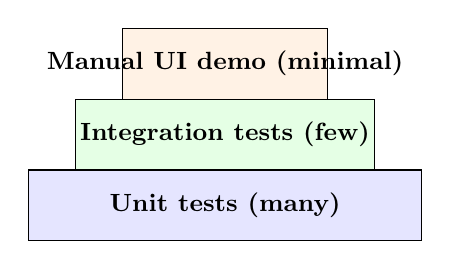
\begin{tikzpicture}[every node/.style={font=\small}]
    \draw[fill=blue!10, draw=black] (0,0) rectangle (5,0.9);
    \draw[fill=green!10, draw=black] (0.6,0.9) rectangle (4.4,1.8);
    \draw[fill=orange!10, draw=black] (1.2,1.8) rectangle (3.8,2.7);

    \node at (2.5,0.45) {\textbf{Unit tests (many)}};
    \node at (2.5,1.35) {\textbf{Integration tests (few)}};
    \node at (2.5,2.25) {\textbf{Manual UI demo (minimal)}};
  \end{tikzpicture}
  \slidesources{\OOPSUnitVISources}
\end{frame}

\begin{frame}{JUnit 5 essentials}
  \begin{itemize}[<+->]
    \item Use \texttt{@Test} methods; follow Arrange--Act--Assert.
    \item Assertions: \texttt{assertEquals}, \texttt{assertTrue}, \texttt{assertThrows}.
    \item Use \texttt{@BeforeEach} to set up a clean fixture.
  \end{itemize}
  \slidesources{\OOPSUnitVISources}
\end{frame}

\begin{frame}[fragile]{Example: \texttt{assertThrows} for validation}
\begin{lstlisting}
@Test
void rejectsEndBeforeStart() {
    assertThrows(ValidationException.class,
        () -> service.createBooking(1, "A", 10, 10));
}
\end{lstlisting}
  \begin{itemize}[<+->]
    \item Good tests are small and check one behavior.
    \item Name tests like a sentence: \texttt{rejectsEndBeforeStart}.
  \end{itemize}
  \slidesources{\OOPSUnitVISources}
\end{frame}

\begin{frame}{Design for testability: interface + fake}
  \centering
  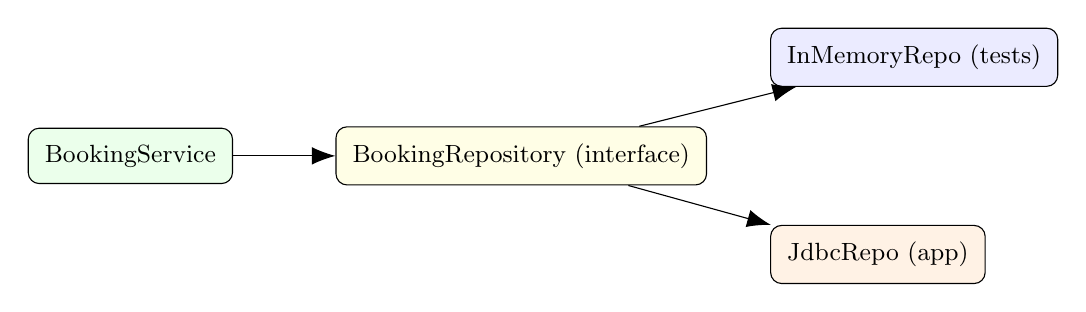
\begin{tikzpicture}[node distance=1.3cm, every node/.style={font=\small}]
    \node[draw, rounded corners, fill=green!8, inner sep=6pt] (svc) {BookingService};
    \node[draw, rounded corners, fill=yellow!10, right=of svc, inner sep=6pt] (iface) {BookingRepository (interface)};
    \node[draw, rounded corners, fill=blue!8, above right=0.5cm and 0.8cm of iface, inner sep=6pt] (fake) {InMemoryRepo (tests)};
    \node[draw, rounded corners, fill=orange!10, below right=0.5cm and 0.8cm of iface, inner sep=6pt] (jdbc) {JdbcRepo (app)};
    \draw[-{Latex[length=3mm]}] (svc) -- (iface);
    \draw[-{Latex[length=3mm]}] (iface) -- (fake);
    \draw[-{Latex[length=3mm]}] (iface) -- (jdbc);
  \end{tikzpicture}

  \vspace{0.6em}
  \begin{itemize}[<+->]
    \item Tests run fast without DB.
    \item Production uses JDBC implementation.
  \end{itemize}
  \slidesources{\OOPSUnitVISources}
\end{frame}

\begin{frame}{Integration checklist (DAO + DB)}
  \begin{enumerate}[<+->]
    \item Run \texttt{schema.sql} on a clean DB.
    \item Insert one row using DAO.
    \item List/find and verify mapping fields.
    \item Update and verify changes.
    \item Delete and verify removal.
  \end{enumerate}
  \slidesources{\OOPSUnitVISources}
\end{frame}

\begin{frame}{Build + packaging (idea)}
  \begin{itemize}[<+->]
    \item Maven: \texttt{mvn test}, then \texttt{mvn package} (Jar in \texttt{target/})
    \item Gradle: \texttt{gradle test}, then \texttt{gradle build}
    \item Artifact should be runnable with clear instructions.
  \end{itemize}
  \textbf{Tip:} record your run steps in README (so TA can run it quickly).
  \slidesources{\OOPSUnitVISources}
\end{frame}

\begin{frame}{Release + demo preparation}
  \begin{itemize}[<+->]
    \item Freeze scope: choose what you will demo.
    \item Run tests + integration checklist.
    \item Prepare demo data (1--2 example resources, bookings).
    \item Create a release (tag) and attach the artifact.
  \end{itemize}
  \slidesources{\OOPSUnitVISources}
\end{frame}

\section{Demo / Example}
\label{sec:demo}

\begin{frame}{Demo script (5--7 mins)}
  \begin{enumerate}[<+->]
    \item Start DB; confirm schema exists.
    \item Run the app; show one end-to-end flow (Add Resource $\rightarrow$ list).
    \item Show booking flow (create + list).
    \item Show validation (invalid booking shows a clean message).
    \item (Optional) Run tests: \texttt{mvn test}.
  \end{enumerate}
  \slidesources{\OOPSUnitVISources}
\end{frame}

\begin{frame}{Mini Exercises (5 mins)}
  \begin{enumerate}[<+->]
    \item Write one unit test for a service rule in your project.
    \item What is one integration test you must do for DAO?
    \item What 3 steps should be in your README ``How to run''?
  \end{enumerate}
  \slidesources{\OOPSUnitVISources}
\end{frame}


\section{Summary}
\label{sec:summary}

\begin{frame}{Key Takeaways}
  \begin{itemize}[<+->]
    \item Test service rules with JUnit; keep tests fast and focused.
    \item Verify DAO with an integration checklist.
    \item Package a runnable artifact and rehearse a short demo script.
  \end{itemize}
  \slidesources{\OOPSUnitVISources}
\end{frame}

\begin{frame}{Checkpoint Questions}
  \begin{enumerate}[<+->]
    \item What is the difference between unit and integration tests?
    \item Why does ``depend on an interface'' help testing?
    \item What must be included in a demo-ready release artifact?
  \end{enumerate}
  \slidesources{\OOPSUnitVISources}
\end{frame}

\begin{frame}{Course Wrap-Up}
  \begin{itemize}[<+->]
    \item Use OOP principles to keep code clean and reusable.
    \item Use interfaces and layering to reduce coupling.
    \item Use testing + packaging to ship reliable software.
  \end{itemize}
  \slidesources{\OOPSUnitVISources}
\end{frame}

\end{document}
